\documentclass[tikz,border=8pt]{standalone}
% Shared look for every TikZ diagram. Load with \input{../../tools/tikz-style.tex}
\usepackage[T1]{fontenc}
\usepackage{lmodern}
\renewcommand{\sfdefault}{lmr}  % diagrams use the same serif as the text
\usetikzlibrary{arrows.meta, positioning, shapes.geometric, calc, fit, backgrounds}
\definecolor{cblue}{HTML}{4C78A8}
\definecolor{corange}{HTML}{F58518}
\definecolor{cgreen}{HTML}{54A24B}
\definecolor{cred}{HTML}{E45756}
\definecolor{cpurple}{HTML}{B279A2}
\definecolor{cgrey}{HTML}{6B6B6B}
\tikzset{
  every picture/.style={font=\sffamily, line width=1.2pt},
  box/.style={draw=#1, fill=#1!12, rounded corners=4pt, align=center, inner sep=7pt, minimum height=1.1cm},
  box/.default=cgrey,
  arrow/.style={-{Stealth[length=3mm]}, draw=cgrey, line width=1.4pt},
  title/.style={font=\sffamily\bfseries\Large},
  note/.style={font=\sffamily\small, text=cgrey, align=center},
}
\AtBeginDocument{\hyphenpenalty=10000 \exhyphenpenalty=10000}

\begin{document}
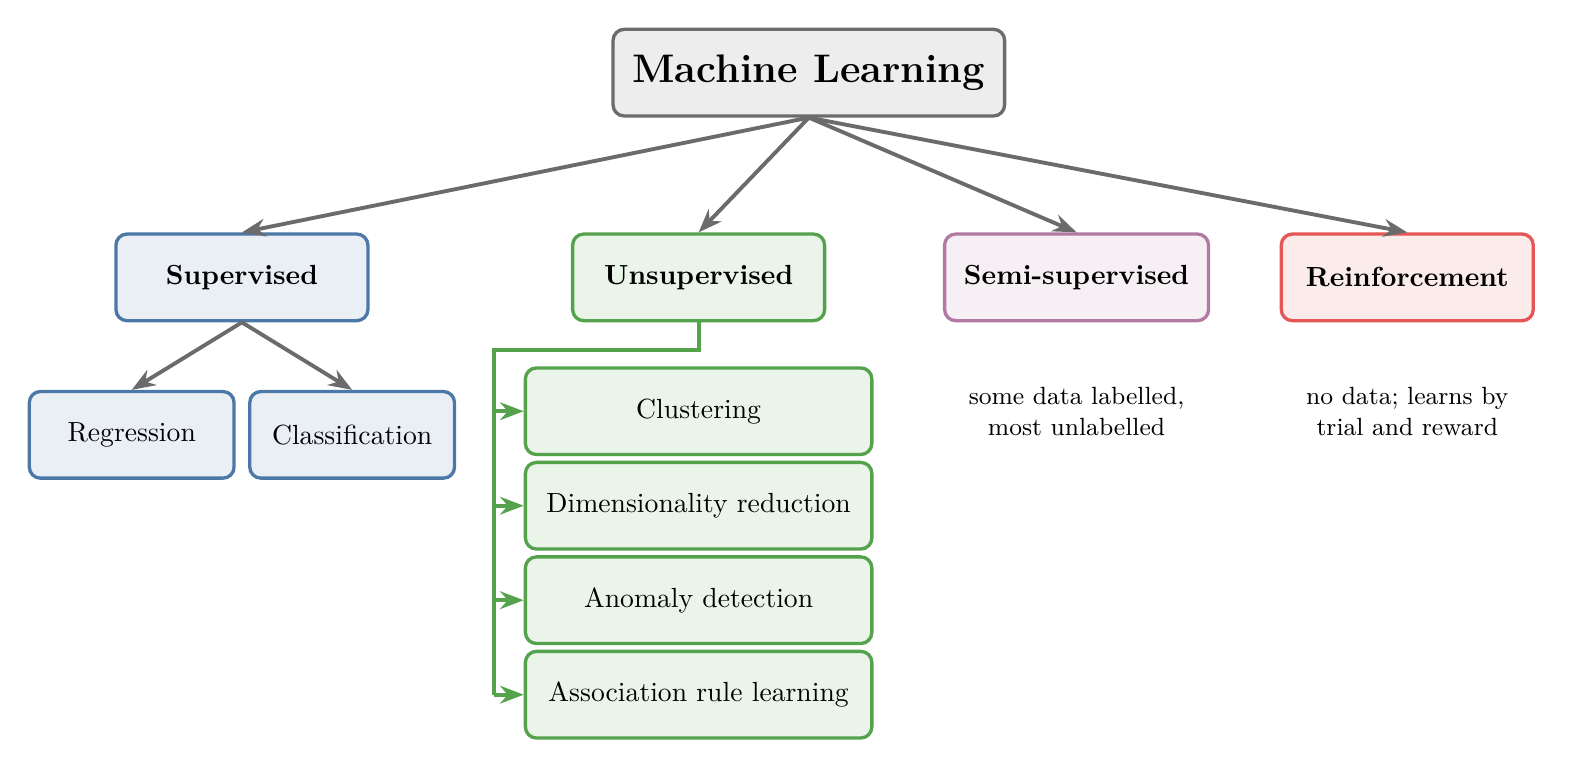
\begin{tikzpicture}
  \node[box=cgrey, font=\sffamily\bfseries\Large] (ml) at (0,0) {Machine Learning};
  \node[box=cblue,   minimum width=3.2cm, font=\sffamily\bfseries] (sup)  at (-7.2,-2.6) {Supervised};
  \node[box=cgreen,  minimum width=3.2cm, font=\sffamily\bfseries] (uns)  at (-1.4,-2.6) {Unsupervised};
  \node[box=cpurple, minimum width=3.2cm, font=\sffamily\bfseries] (semi) at ( 3.4,-2.6) {Semi-supervised};
  \node[box=cred,    minimum width=3.2cm, font=\sffamily\bfseries] (rl)   at ( 7.6,-2.6) {Reinforcement};
  \foreach \n in {sup,uns,semi,rl} \draw[arrow] (ml.south) -- (\n.north);
  \node[box=cblue, minimum width=2.6cm] (reg) at (-8.6,-4.6) {Regression};
  \node[box=cblue, minimum width=2.6cm] (cls) at (-5.8,-4.6) {Classification};
  \draw[arrow] (sup.south) -- (reg.north); \draw[arrow] (sup.south) -- (cls.north);
  \node[box=cgreen, minimum width=4.4cm] (u1) at (-1.4,-4.3) {Clustering};
  \node[box=cgreen, minimum width=4.4cm] (u2) at (-1.4,-5.5) {Dimensionality reduction};
  \node[box=cgreen, minimum width=4.4cm] (u3) at (-1.4,-6.7) {Anomaly detection};
  \node[box=cgreen, minimum width=4.4cm] (u4) at (-1.4,-7.9) {Association rule learning};
  \draw[cgreen, line width=1.4pt] (uns.south) -- ++(0,-0.35) -| (-4.0,-7.9);
  \foreach \u in {u1,u2,u3,u4} \draw[arrow, draw=cgreen] (-4.0,0 |- \u) -- (\u.west);
  \node[note, text=black, text width=3.4cm] at (3.4,-4.3) {some data labelled,\\most unlabelled};
  \node[note, text=black, text width=3.4cm] at (7.6,-4.3) {no data; learns by\\trial and reward};
\end{tikzpicture}
\end{document}
